\chapter{System Development}
\section{Subsystems}

The system will be split up into a number of subsystems, shown
in~\cref{fig:subsystems}. Each of these subsystems is described in more detail
in the sections below, and a brief description is given immediately below.

\begin{itemize}

  \item Two analogue input channels come into the system, and are amplified and
  offset by amplification circuitry (with the gain controlled by a central
  microcontroller).

  \item These channels are both sampled using an Analogue to Digital Converter,
  which feeds into the microcontroller.

  \item A number of digital inputs are also fed straight into the
  microcontroller

  \item Through a Bluetooth transceiver, an Android device interacts with the
  microcontroller, receiving samples of both the analogue and digital inputs and
  controlling things such as the sampling rate and amplifier gain.

\end{itemize}

\begin{landscape}
  \begin{figure}
    \scalebox{0.8}{
      \begin{tikzpicture}
        \node [io] (input1) {Input 1};
        \node [io, below of=input1, node distance=3cm] (input2) {Input 2};

        \node [process, right of=input1] (amp1) {Amplifier};
        \node [process, right of=input2] (amp2) {Amplifier};
        \path [arrow] (input1) -- (amp1);
        \path [arrow] (input2) -- (amp2);
        \coordinate [below of=amp1, node distance=1.5cm] (centreamp);

        \node [process, right of=centreamp] (adc) {ADC};
        \path [arrow] (amp1) -| (adc);
        \path [arrow] (amp2) -| (adc);

        \node [process, right of=adc] (microcontroller) {Microcontroller};
        \path [barrow] (adc) -- (microcontroller);

        \node [process, below=2.5cm of microcontroller.320] (inputdigital) {Digital Inputs};
        \path [arrow] (inputdigital) -- (microcontroller.320);

        \node [process, right of=microcontroller] (wifi) {Bluetooth Transceiver};
        \node [io, right of=wifi, node distance=5.5cm, text width=4.5em] (frontend) {User Interface};
        \path [barrow] (microcontroller) -- (wifi);
        \path [bdarrow] (wifi) -- (frontend);

        \coordinate[above of=amp1, node distance=2cm] (aboveamp1);
        \coordinate[below of=amp2, node distance=1.5cm] (belowamp2);
        \path [arrow] (microcontroller) |- (aboveamp1) -- (amp1);
        \path [arrow] (microcontroller.220) |- (belowamp2) -- (amp2);
      \end{tikzpicture}
    }
    \caption[Oscilloscope Subsystems]{Subsystems within the oscilloscope}
    \label{fig:subsystems}
  \end{figure}
\end{landscape}

\subsection{Analogue Inputs}

For the purposes of this project wires are sufficient, however in a real-life
scenario high-impedance, low-inductance test probes (usually coaxial cable)
should be used.

\subsection{Amplifiers}

Each amplifier will have two purposes:
\begin{itemize}
  \item To amplify the signal based on the Voltage Control of the oscilloscope.
    This is needed so the user can input a range of different voltage signals.

  \item To shift the signal so the minimum voltage is \SI{0}{\volt}, rather
    than some negative voltage. This is required because the ADC will only
    accept an input greater than \SI{0}{\volt}.
\end{itemize}

The chosen ADCs require an input voltage between \SI{0}{\volt} and
\SI{5}{\volt}\footnote{The maximum voltage is actually $V_{REF+}$, which will be
connected to $V_{CC}$ for simplicity, which in this case is \SI{5}{\volt}}. A
non-inverting summing amplifier would not be suitable beause the offset added to
the signal needs to remain constant while the gain changes, so instead the
amplifier will be split into two stages.

The first stage will amplify the signal and offset it to be between
\SI{0}{\volt} and \SI{-5}{\volt}, below which the op-amp will saturate.

The second stage will invert this signal with a voltage gain of $-1$, meaning
the output voltage will be between \SI{0}{\volt} and \SI{5}{\volt} as required.

\subsubsection{First Stage}

\paragraph{Circuit}
This stage will be implemented using a summing amplifier, with the inputs
consisting of the input signal and a fixed voltage (for the sake of simplicity,
the 5V supply wil be used).

See~\cref{fig:first_stage_amplifier_circuit} for a circuit diagram.

\paragraph{Component Calculations}

Suppose that the input signal varies from $-V_1$ to $+V_1$, and the amplifier
has a gain of $A$ and an offset of $B$. Then the output voltage $V_o$ will be
given by

\begin{equation*}
  -V_o = \frac{R_f}{R_1} V_i + \frac{R_f}{R_2} \cdot \SI{5}{\volt}
\end{equation*}

The first term will range from $-A\cdot V_1$ to $+A\cdot V_1$, and the second
term will be $B$. So $-V_o$ will range from $B-A\cdot V_1$ to $B+A\cdot V_1$.
Choosing a value of $B=\SI{2.5}{\volt}$ means that $-V_o$ will vary equally
above and below \SI{2.5}{\volt}, as we want\footnote{The op amp will saturate
before outputting a voltage above \SI{5}{\volt}, so we don't need to worry about
this. If the gain or input voltage is sufficiently large, $-V_o$ could fall
below \SI{0}{\volt}. This means the next stage must saturate at $\SI{0}{\volt}$
and not output negative voltages, whatever the input.  }(because the voltage
must be between \SI{0}{\volt} and \SI{5}{\volt}, and \SI{2.5}{\volt} is the
midpoint of those two).

$R_f$ and $R_2$ will be fixed to give $\frac{R_f}{R_2}=0.5$ to get the required
offset. $R_1$ will be a digital potentiometer acting as a rheostate (variable
resistor), allowing the microcontroller to control the gain of the amplifier.

The input voltage range is from \SI{\pm 50}{\mV} to \SI{\pm 5}{\V}, so the gain
$A=\frac{R_f}{R_1}$ must vary from 0.5 to at least 50.  Digital potentiometers
are readily available in a number of values, so the standard \SI{10}{\kilo\ohm}
option will be chosen. This means the potentiometer can vary from the minimum
resistance (usually \SI{75}{\ohm}) to \SI{10}{\kilo\ohm}.

Using the values for $A$ and $R_1$, this gives a value of
$R_f=\SI{5}{\kilo\ohm}$, meaning $A$ will range from
$\frac{\SI{5}{\kilo\ohm}}{\SI{10}{\kilo\ohm}}=0.5$ to
$\frac{\SI{5}{\kilo\ohm}}{\SI{75}{\ohm}} \approx 66.7$, as required.  In turn,
this gives a value of $R_2 = \SI{10}{\kilo\ohm}$.

\begin{figure}[ht]
  \begin{circuitikz}[european]
    % Inputs and input resistors
    \node (vin1) {};
    \node (vin2) [below=1 of vin1] {};
    \node (rpoint1) [right=2.5 of vin1] {};
    \node (rpoint2) [right=2.5 of vin2] {};
    \coordinate (middlevin1vin2) at ($(vin1)!0.5!(vin2)$);
    \node (rpoint) at (rpoint1|- middlevin1vin2) {};

    \draw (vin1) to[R, l=$R_2\equal\SI{10}{\kilo\ohm}$] (rpoint1);
    \draw (rpoint2) to[pR, l_=$R_1 \in \lb\SI{75}{\ohm}\comma
    \SI{10}{\kilo\ohm}\rb$, label/align=rotate, -o] (vin2) node [anchor=east]{$V_{in}$};
    \draw (rpoint1) to[short] (rpoint);
    \draw (rpoint2) to[short] (rpoint);
    \node [circ] (crpoint) at (rpoint) {};

    % Op amp and feedback resistor
    \node (rfpoint) [right=1 of rpoint] {};
    \node[op amp](oa) [right=0.5 of rfpoint] {};
    \node (aboverfpoint) [above=1.5 of rfpoint] {};
    \node (2xaboverfpoint) [above=1.5 of aboverfpoint] {};
    \node (aboveoaout) at (oa.out|- aboverfpoint) {};
    \node[ground](gnd) [below=0.5 of rfpoint,anchor=center] {};
    \node (vo) [right=1 of oa.out] {};

    \draw (rpoint) to[short] (rfpoint);
    \draw (rfpoint) to[short] (aboverfpoint);
    \draw (aboverfpoint) to[R=$R_f\equal\SI{5}{\kilo\ohm}$] (aboveoaout);
    \draw (aboveoaout) to[short] (oa.out);
    \node [circ] (crfpoint) at (rfpoint|- oa.-) {};

    \draw (rfpoint) |- (oa.-);
    \draw (gnd) |- (oa.+);
    \draw (oa.out) to[short] (vo) node [anchor=west] {$V_{out}$};

    % 5V rail
    \node (leftofvin1) [left=0.5 of vin1] {};
    \node (5vraill) at (leftofvin1|- 2xaboverfpoint) {};
    \node (5vrailr) [right=3 of 5vraill] {};
    \node (5vrailm) at (vin1|- 5vraill) {};

    \draw (5vraill) to[short] (5vrailr) node [anchor=west] {$\SI{5}{\volt}$};
    \draw (5vrailm) to[short] (vin1);
  \end{circuitikz}
  \caption[1\ts{st} Amplifier Stage]{First stage amplifier circuit diagram}
  \label{fig:first_stage_amplifier_circuit}
\end{figure}

\paragraph{Component Selection}

The Microchip MCP4131-103E/P will be used for the digital potentiometer. It
offers enough precision (typically 0.25\%), offers a simple interface for
changing the resistance (SPI) and is cheap and readily available in a PDIP
package. Additionally, free samples are available from Microchip. To make the
component calculations made earlier work, the \SI{10}{\kilo\ohm} MCP4131-103
variety will be used.

The op-amps should be of rail-to-rail type (i.e. they can saturate at almost 0V
and $V_s$) and be able to cope with $V_s=\SI{5}{\volt}$, $V_i=\SI{5}{\volt}$ and
input frequencies of up to $\SI{1}{\MHz}$. The Analog Devices AD8031 meets all
of these requirements (at $\SI{1}{\MHz}$ it gives an open-loop gain of almost
$\SI{25}{\decibel}$) and is also cheap and readily available in PDIP packaging.
Due to the availability of free samples, 2 AD8032ANZs (consisting of two AD8031
op amps in each chip) will be used.

\subsubsection{Second Stage}
This stage simply has to invert the previous stage, saturating at \SI{0}{\volt}
and \SI{5}{\volt}. For this we can use a simple inverting amplifier.

\begin{equation*}
V_{out}=\frac{R_f}{R_1}V_{in}
\end{equation*}

Choosing a standard value of $R_f=\SI{10}{\kilo\ohm}$, we obtain
$R_1=\SI{10}{\kilo\ohm}$.

As detailed in the previous section, AD8031 op amps will be used.

See~\cref{fig:second_stage_amplifier_circuit} for a circuit diagram.

\begin{figure}[ht]
  \begin{circuitikz}[european]
    \node (vin) {};
    \node (rpoint) [right=2.5 of vin] {};
    \node [op amp] (oa) [right=0.5 of rpoint] {};
    \node (aboverpoint) [above=1.5 of rpoint] {};
    \node (aboveoaout) at (oa.out |- aboverpoint) {};
    \node [ground] (gnd) [below=0.5 of rpoint, anchor=center] {};
    \node (vo) [right=1 of oa.out] {};


    \draw (rpoint) to[R, l_=$R_1\equal\SI{10}{\kilo\ohm}$] (vin) node
      [anchor=east] {$V_{in}$};
    \node [circ] (crpoint) at (rpoint|- oa.-) {};
    \draw (rpoint) to[short] (aboverpoint);
    \draw (aboverpoint) to [R=$R_f\equal\SI{10}{\kilo\ohm}$] (aboveoaout);
    \draw (aboveoaout) to[short] (oa.out);
    \draw (rpoint) |- (oa.-);
    \draw (gnd) |- (oa.+);
    \draw (oa.out) to[short] (vo) node [anchor=west] {$V_{out}$};
  \end{circuitikz}
  \caption[2\ts{nd} Amplifier Stage]{Second stage amplifier circuit diagram}
  \label{fig:second_stage_amplifier_circuit}
\end{figure}

\subsubsection{Simulation}
To check the frequency response of the amplification circuit, it was simulated
using LTSpice (see~\cref{fig:amp_sim:circuit}).

To test the simulation, a low frequency sine wave was applied, and as expected
the output was a sine wave of amplitude \SI{2.5}{\volt} between \SI{0}{\volt}
and \SI{2.5}{\volt}. The resultant waveform can be seen
in~\cref{fig:amp_sim:waveform}. A FFT was then applied to this waveform to
obtain the frequency spectrums seen in~\cref{fig:amp_sim:fft}. As required, the
spectrum of the output was identical to the spectrum of the input, with the
slightly lower amplitudes being due to a lower wave amplitude (\SI{2.5}{\volt}
c.f. \SI{5}{\volt}).

A frequency sweep was then applied to produce a Bode plot. The details of such a
plot are beyond the scope of this project, but let us just note that the gain is
very consistent across all frequencies we'll be using (as predicted: the op amp
has a stated bandwidth of \SI{80}{\MHz}, much higher than \SI{1}{\MHz}), and
while it becomes almost \SI{9}{\degree} out of phase at very high frequencies,
this is not an issue for this project\footnote{The phase is only important to
the oscilloscope when comparing the phase of two signals. To see two signals on
screen at the same time base, their frequencies must be close enough together
that they're both out of phase by approximately the same amount. Hence their
phase difference is unchanged}.

\begin{figure}[ht]
  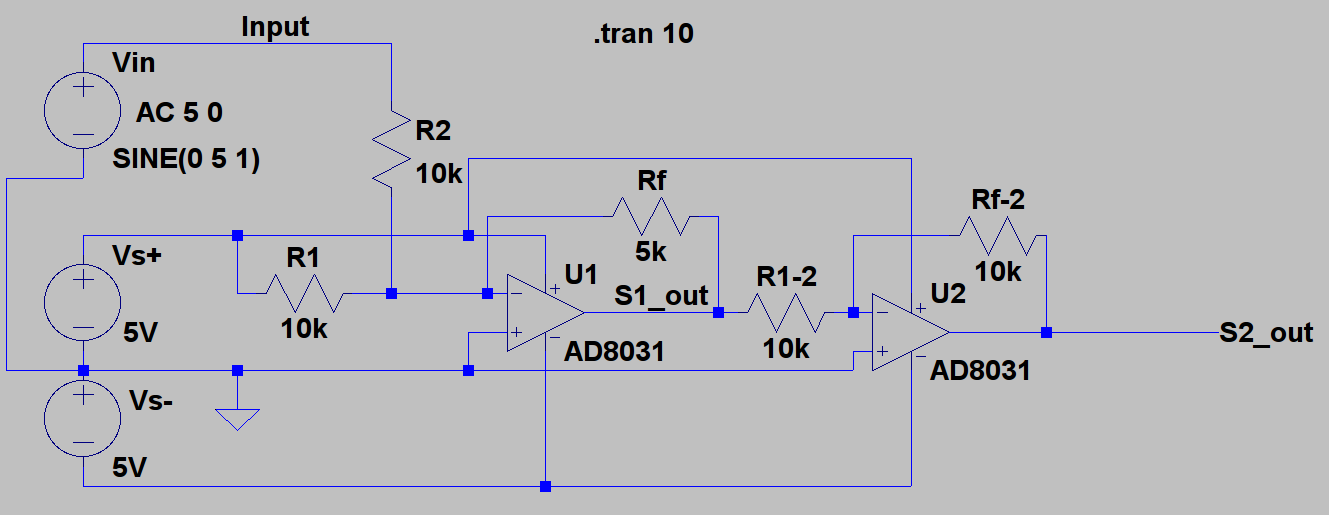
\includegraphics[width=\textwidth]{img/amplifier/circuit.png}
  \caption[Amplification Circuit Simulation]{Amplification circuit in LTSpice}
  \label{fig:amp_sim:circuit}
\end{figure}

\begin{landscape}
  \begin{figure}[ht]
    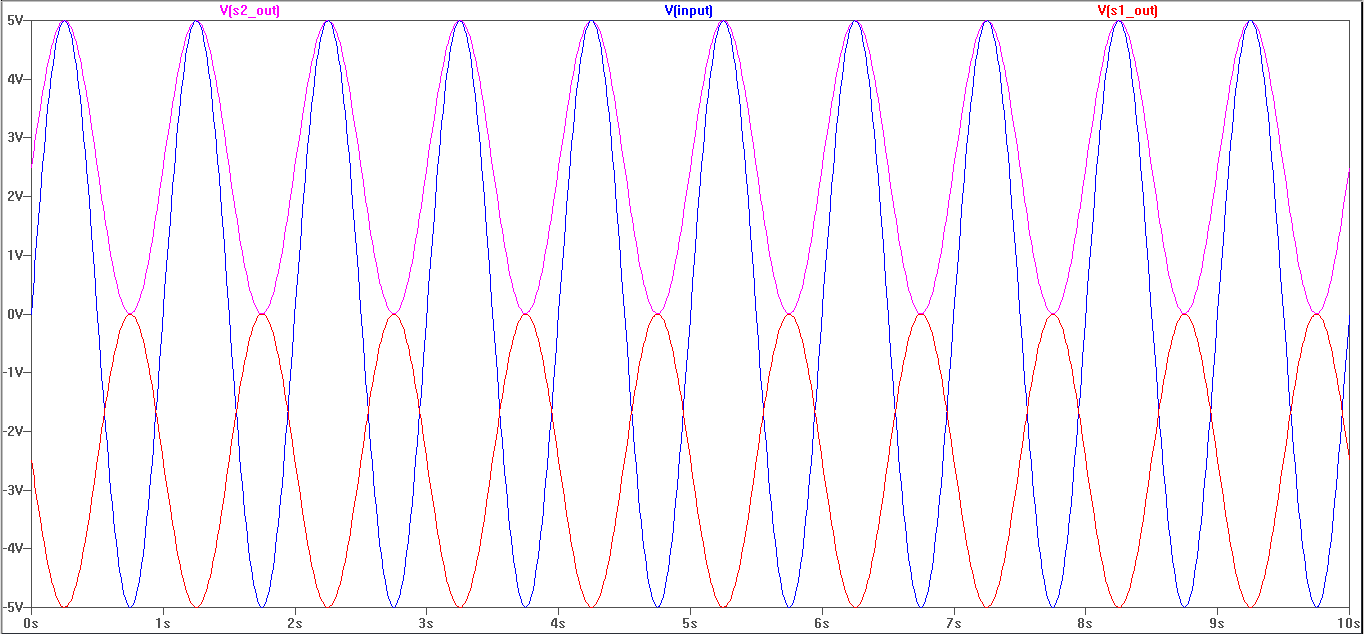
\includegraphics[width=\linewidth]{img/amplifier/waveform_inverted.png}
    \caption[Amplification Circuit Waveform]{Waveform produced by amplification circuit at 1Hz (blue = original,
      red = first stage output, magenta = second stage output)}
    \label{fig:amp_sim:waveform}
  \end{figure}
\end{landscape}

\begin{landscape}
  \begin{figure}[ht]
    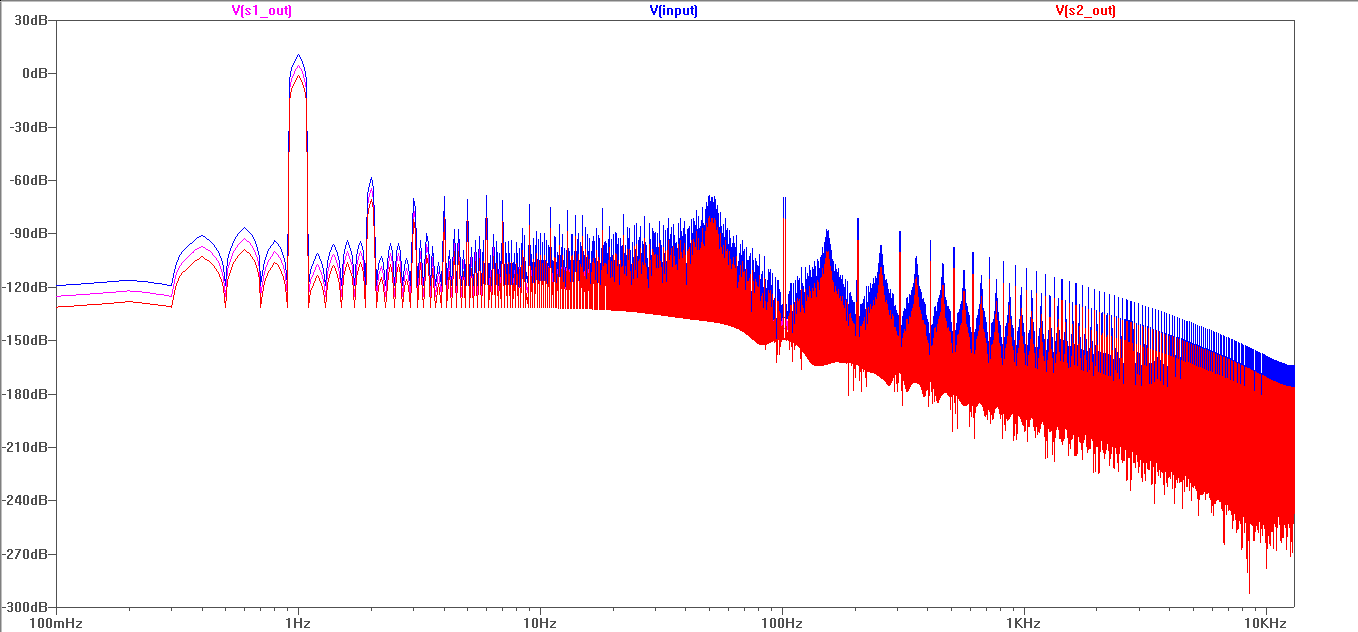
\includegraphics[width=\linewidth]{img/amplifier/fft_inverted.png}
    \caption[Amplification Circuit Frequency Spectrum]{FFT of waveform produced by amplification circuit at 1Hz (red =
      original, blue = first stage output, magenta = second stage output)}
    \label{fig:amp_sim:fft}
  \end{figure}
\end{landscape}

\begin{landscape}
  \begin{figure}[ht]
    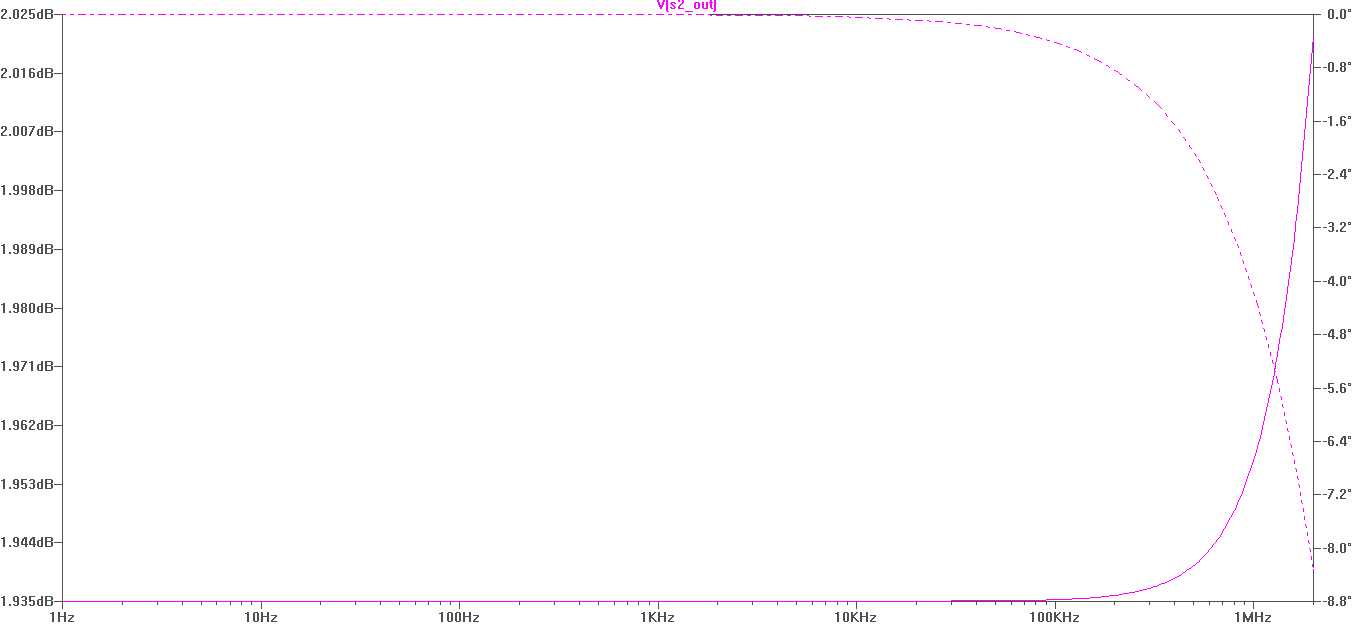
\includegraphics[width=\linewidth]{img/amplifier/frequency_response_inverted.png}
    \caption[Amplification Circuit Bode Plot]{Frequency response of amplification circuit}
    \label{fig:amp_sim:freq_response}
  \end{figure}
\end{landscape}


\subsection{ADCs}
\label{sec:adcs}

As discussed before, these should be able to sample at up to $\SI{1}{\MHz}$. The
only readily available ADCs that can do this in PDIP packaging and have free
samples are the 8-bit half-flash\footnote{Similar to flash ADCs, but requiring
$\approx2^{\frac{n}{2}}$ as opposed to $\approx 2^n$ parts} Maxim Integrated
MAX114 ADCs.

There are a number of modes the ADCs can be operated in, however the pipelined
mode offers a very good compromise between complexity and speed. The full
details are in \textcite{MAX114}, but as the ADCs are operated from a
microcontroller in which there's a delay of \SI{62.5}{\ns} (assuming a
\SI{16}{\MHz} clock) between each instruction, the operating procedure can be
simplified to the following:

\begin{enumerate}
  \item Use $A_0$ and $A_1$ to choose the input signal ($00$ for input 0, $01$
  for input 1, the only two inputs used in this project)
  \item Pull $\overline{CS}$, $\overline{RD}$ and $\overline{WR}$\footnote{For
  simplicity, $\overline{CS}$, $\overline{RD}$ and $\overline{WR}$ can all be
  physically tied together and connected to just one microcontroller input} low
  \item Wait approximately \SI{250}{\ns}
  \item Pull $\overline{CS}$, $\overline{RD}$ and $\overline{WR}$ back high
  \item Read in a sample from $D_0$ through $D_7$
\end{enumerate}

Taken directly from the datasheet, \cref{fig:MAX114Power} shows the connections
that must be made to power the MAX114 and provide it with a reference voltage.

Additionally, $\overline{PWRDN}$ must be kept high to keep the ADC powered on,
and $MODE$ must be kept high to keep the ADC in Read-Write mode (of which
pipeline mode is a subset).

\begin{figure}
  \centering
  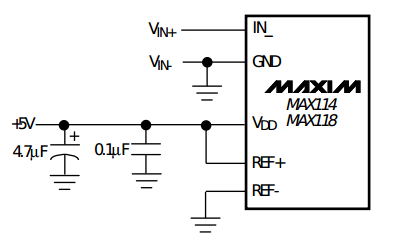
\includegraphics[width=0.4\textwidth]{img/adc/max114power.png}
  \label{fig:MAX114Power}
  \caption[ADC Power Connections]{Power connections for the MAX114~\autocite{MAX114}}
\end{figure}


\subsection{Microcontroller}

Due to this author's significant previous experience with AVR microcontrollers,
one will be used as there are no significant disadvantages over a PIC. The main
requirements the microcontroller needs to satisfy are:

\begin{itemize}
  \item Ability to use a \SI{16}{\MHz} clock
  \item Inbuilt UART communication (to communicate with the Bluetooth module)
  \item A significant number (at least 20) input/output pins
  \item At least \SI{1}{\kilo byte} of SRAM (to store the 8192 bits of samples)
  \item Availability in a PDIP package
\end{itemize}

The ATMega328 (more commonly known as the chip powering most Arduinos) was
chosen because it satisfies all of these requirements and this author had a
number of spare chips not being used.

\subsubsection{Circuit}
For the chip to operate, a \SI{16}{\MHz} crystal oscillator must be connected
between $XTAL1$ and $XTAL$, with a \SI{22}{\pF} capacitor from each pin to
ground. Additionally, the following power connections must be made:

\begin{itemize}
  \item $RESET$ to \SI{5}{\volt} through a \SI{10}{\kilo\ohm} resistor
  \item Both $GND$s to ground
  \item $VCC$ and $AVCC$ to \SI{5}{\volt}
\end{itemize}

To program the chip, an AVR programmer must be used. These are available very
cheaply (such as the USBASP for \pounds 5 from eBay), but an Arduino
(essentially a microcontroller development board) can also be used, as shown
in~\cref{fig:arduino_programmer}. As this author had a spare Arduino, this
option was used.

\begin{figure}
  \centering
  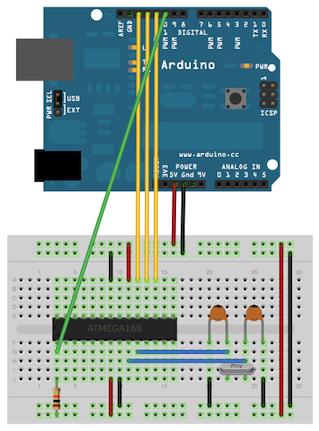
\includegraphics[width=0.5\textwidth]{img/microcontroller/arduino_programmer.png}
  \label{fig:arduino_programmer}
  \caption[Arduino as a Programmer]{Breadboard diagram produced by~\textcite{ArduinoProgrammer} showing
  the programming and power connections between an Arduino and an ATMega328}
\end{figure}


\subsubsection{Serial Interface}

The following protocol was designed for serial communication between the Android
device and the microcontroller. After taking a full 1024 samples, the
microcontroller checks the serial buffer for one of the following commands and
acts on it, responding via serial if necessary.

Traditionally, serial is a textual interface, however for efficiency's sake in
this case it was used as a binary interface. Each transmitted character is
stored as an 8-bit character, so the protocol is based on the integer values of
those characters. For example, 65 below corresponds to a capital `A'.

\begin{description}

  \item[\texttt{0x00}] Return all samples for the first analogue channel (1024
  bytes, followed by a newline.\footnote{The character used to indicate a new
  line should start in text on a computer. Here, it's just equivalent to
  \texttt{0x0A}})

  \item[\texttt{0x01}] Return all samples for the second analogue channel (1024
  bytes, followed by a newline)

  \item[\texttt{0x02}] Wait for the next transmitted byte, $X$, and return all
  values for the $X$th digital channel (1024 bits = 128 bytes, followed by a
  newline)

  \item[\texttt{0x03}] Use analogue channel 1 to trigger (returns a newline)

  \item[\texttt{0x04}] Use analogue channel 2 to trigger (returns a newline)

  \item[\texttt{0x05}] Wait for the next transmitted byte, $X$, and use the
  $X$th digital channel to trigger (returns a newline)

  \item[\texttt{0x06}] Wait for the next two transmitted bytes, $X$ and $Y$ and
  use $XY$\footnote{For example, if $X = \texttt{0x50}$ and $Y=\texttt{0x1A}$
  then use \texttt{0x501A} as the delay} as the number of microseconds to pause
  in between samples (returns a newline)

  \item[\texttt{0x07}] Wait for the next transmitted byte, $X$, and use $X$ as
  the analogue trigger threshold (returnsa  newline)

  \item[\texttt{0x08}] Wait for the next transmitted byte, $X$, and use the 7
  least significant bits of $X$ as the digital pot value in an amplifier (if the
  most significant bit of $X$ is high, the second amplifier circuit, otherwise
  the first amplifier circuit) (returns a newline)

  \item[\texttt{0x09}] Enable analogue channels 1 and 2 (this means slower
  sampling) (returns a newline)

  \item[\texttt{0x0A}] Noop (this is the newline character) (returns a newline)

  \item[\texttt{0x0B}] Enable analogue channel 1 only (faster sampling)
  sampling) (returns a newline)

\end{description}

So, for example, to receive samples for the second analogue channel the Android
device would have to send \texttt{0x01}, then store the next 1024 received bytes.

\subsubsection{ADC Communication}
The way in which the microcontroller will communicate with the ADC is described
in~\cref{sec:adcs}.

\subsubsection{Digital Potentiometer Commmunication}

The resistance of the digital potentiometers is set using an SPI interface.
While the details can get more complicated, SPI (Serial Peripheral Interface) is
essentially a very simple interface, consisting of four pins: $SCLK$, $MOSI$,
$MISO$ and $\overline{SS}$.

There are two devices: a master and a slave. $SCLK$ is simply a clock output
from master. On either the rising or falling edge of $SCLK$, a bit of data is
transmitted from master to slave on $MOSI$ and slave to master on $MISO$.
$\overline{SS}$ is simply an active low slave select (i.e. the slave only
communicates when $\overline{SS}$ is low).

There are four different SPI modes, of which the digital potentiometers support
two ($CPOL=0=CPHA$ and $CPOL=1=CPHA$). In both modes, data is captured on the
rising edge and propogated on the falling edge. The difference is simply the
first value of the clock: in the first mode, it's low, and in the second it's
high.

The maximum clock supported by the digital potentiomers is \SI{10}{\MHz}, which
is faster than we can reliably communicate at with a \SI{16}{\MHz}
microcontroller anyway.

To send a 16-bit byte to the digital potentiometer the following must be done:
\begin{enumerate}
  \item Pull $\overline{SS}$ low
  \item Wait one $SCLK$ period
  \item Starting from a high (an artbitrary choice), pulse $SCLK$
  \item On each falling edge, send a bit of data until 16 bits have been sent
  \item Pull $SCLK$ back high
  \item Wait one clock period
  \item Pull $\overline{SS}$ back high
\end{enumerate}

\fxwarning{More on digital pot. communication}

\subsubsection{Program}
To perform all of the above tasks, then, the microcontroller will need to run
the following program:

\begin{itemize}
  \item Loop forever:
    \begin{itemize}
      \item Loop 1024 times:
        \begin{itemize}
          \item Take sample from first analog channel
          \item Take sample from second analog channel, if enabled
          \item Take 1-bit sample from each digital channel
        \end{itemize}
      \item Look at most recent serial command, and perform any actions and send
      any data it specifies
      \item Clear most recent serial command
    \end{itemize}
  \item Interrupt on serial byte received:
    \begin{itemize}
      \item Store as most recent serial command
      \item Receive up to 2 more bytes depending on the command
    \end{itemize}
\end{itemize}


\subsection{Bluetooth Transceiver}
\label{sec:wireless_transceiver}

As discussed in~\cref{sec:CommOptions}, Bluetooth was chosen to communicate with
the Android device acting as the user interface. In particular, the JY-MCU HC-06
was chosen.

\subsection{User Interface}
\label{sec:user_interface}

A high-quality enough screen that interfaced directly with the microcontroller
would be quite expensive, so instead an Android device was chosen as the user
interface.

Android was chosen over the alternatives (iOS, etc) primarily because it's the
most popular mobile operating system, allowing the greatest number of people to
use the oscilliscope. Additionally, it allows easy and open development, whereas
competitors such as iOS require costly developer licenses, proprietary software
and specific hardware.


\section{Construction}
Initially, a number of the subsystems were built individually on breadboards.
This allowed the basic circuit details to be checked without requiring an
infeasibly large circuit to be built on a breadboard. 

\subsection{PCB Layout}
Once this prototype verification step was performed, the PCB was laid out on a
breadboard. This process consists of three main steps: inputting the schematic
into the computer, laying out the schematic components onto the board and
routing traces (the PCB equivalent of wires) between the components.

Initially this was attempted using a piece of software called Eagle. A
significant number of electronics projects use Eagle, from small hobbyist
projects right up to industrial products. However, as this author started to lay
components onto the PCB using Eagle, one encountered an error: the free version
of Eagle only allows a maximum PCB size of \SI{100}{\mm}x\SI{80}{\mm}. For
reasons discussed later, the PCB size needed to be \SI{100}{\mm}x\SI{100}{\mm}.
The cheapest paid-version of Eagle is \$169, meaning it was much too expensive
to purchase for the sake of this project. Instead, an alternative was sought.

This author researched and briefly evaluated two alternatives: KiCAD and
DipTrace. KiCAD is a piece of open source software, meaning it's free to
use
\footnote{There are two disctinct definitions of free that should be
considered here: gratis free (without cost to the user, this is somewhat
confusingly also called free as in beer) and libre free (without compromise to
the user's liberties, this is also known as free as in speech and essentially
means that the user has the right to run the software however they want, as
well as the right to modify it, meaning the source code is freely available.
Software that's Free (with a capital F) is also known as open-source software
(there are major differences between the two terms, however for the purposes
of this explanation the reader can consider them identical) is both free as in
gratis and free as in libre, and common examples include LibreOffice (hence
the name) and GNU/Linux (the operating system running everything from the
majority of super computers to televisions to traffic lights). For more on this
subject, see Richard Stallman's book `\textit{Free as in Freedom}', which is
also Free and hence freely available on the internet.},
and DipTrace, a commercial piece of software with a free version available
limited to 2 signal layers\footnote{It would be impractical to have all of the
  traces in a PCB in the same horizontal plane, as they would not be able to
  cross at any point. Instead, a number of planes, or \textit{layers}, are used.
  PCBs are made by pressing together a number of 2-sided PCB `chapters`, meaning
  that common numbers of layers are 2, 4 or 6 (with higher numbers possible but
  more expensive). As it's the cheapest available and offers enough trace
routing, a 2 layer board will be used for this project} and 300
pins\footnote{This project uses somewhere in the region of 250 pins, so this
limit is not a problem}.

Both are very capable pieces of software, and KiCAD would certainly be
favourable for philosophical reasons. Howerver, the majority of the ICs used in
the circuit are relatively uncommon. This means that CAD footprints (files
containing the physical dimensions of the chip) are not readily available, so
they must be manually created for each IC instead. This is a much quicker
process in DipTrace than in KiCAD (and indeed than in Eagle), and for this
reason alone DipTrace was chosen.

There were no major issues in creating the circuit schematic in DipTrace,
although a number of revisions were required for small improvements. Laying out
the PCB and routing the traces was much harder. DipTrace contains tools to
automatically place and route, however the electrical engineering community
strongly recommends against using auto routers. Placing and routing is a task
that's extremely hard for a computer to find an optimal solution
to\footnote{There is a classification of such problems, known as NP. Very
  briefly: a \textit{running time} can be assigned to a given algorithm. For
  example, any algorithm to sort a list of numbers is at most
  $\mathcal{O}\left(n\log{n}\right)$, meaning that as the list of numbers grows
  longer, the running time of the algorithm grows slower than $n\log{n}$, where
  $n$ is the length of the list. We say an algorithm is polynomial-time if the
  running time is polynomial (so e.g., it's $\mathcal{O}\left(n^3\right)$ but
  not $\mathcal{O}\left(2^n\right)$). We then say an NP problem is one where the
  solution to the problem can be checked with a polynomial-time algorithm, but
  there is no polynomial-time algorithm to find that solution. An NP-hard
problem is then a problem that is at least as hard as the hardest NP problems.
Routing just one trace, with no obstacles to avoid, is an NP-hard problem}.
While software can make use of heuristics\footnote{A technique designed to find
a good-enough solution to a problem, when finding the optimal one would take too
long}, it's a commonly held belief that even the best autorouting software pales
when compared to a human with a small amount of experience (it may help to think
of PCB routing as art: while a computer can be programmed to come up with pieces
of art, even a small child can create much better ones).

Because of this, your author set about learning how to place and route PCBs. The
American electronics retailer Sparkfun provide a number of online tutorials and
videos regarding PCB routing which were extremely helpful. Eventually, the PCB
was routed, and while an expert would have done much better it sufficed for the
purposes of this project (particularly as there were no high voltages or
high-speed signals ($\ge\SI{50}{\MHz}$) involved). To finish the board, mounting
holes and silkscreen\footnote{The process is just screen printing, which
originally used silk as the screen, hence the name \textit{silkscreen}} (the
explanatory text and markings on a PCB) were added.

\subsection{PCB Production}
The final step in the process was to get the board manufactured. In an American
or European fab house (the name for the company that prints the boards) this
would be extremely expensive. For example, popular EuroCircuits quoted a price
of over over over \pounds 90 to produce just \textbf{one} board.

Instead, a Chinese proxy to a Chinese fab house was chosen (nearly all low cost
Chinese retailers use the Golden Phoenix fab house, but ordering directly from
them requires a minimum order of 100 square inches, far beyond the size of this
project\footnote{The proxies do something called panelisation: group a number of
small boards onto a larger board, have the large board made at a low cost and
then sell on the small boards for a small amount of profit}). DFRobot was chosen
because it offered more affordable delivery options than the other Chinese
options\footnote{EMS post is universally available for only a couple of dollars,
  but can take upwards of a month to arrive as it's simply air mail. Many
  Chinese retailers will also send goods worth hundreds of pounds through EMS
  post, simply writing `\textit{birthday card}` on the side meaning that while
  the retailer doesn't have to pay any export fees there is a high chance of the
  package spending weeks stuck in customs in the UK. Instead, a courier service
was chosen. Most Chinese PCB retailers only offer UPS and FedEx, which would
have cost around \$30 for this order. DFRobot offered DHL as well, which was
just over half the cost at \$16}. The boards cost \$23.99 for 10 boards, with a
\$16 delivery charge on top. At a cost of \$2.40 per board, ordering from a
Chinese retailer made the boards over 60 times cheaper than orderin from a
European fab house!

As required, the boards were \SI{100}{mm}x\SI{100}{mm} and 2 layers. There were
less choices available (the boards hade to be green, and coated in
HASL\footnote{If the boards were to be sold commercially, then HASL couldn't be
  used as it contains lead so breaks the EU Restriction of Hazardous Substances
  Directive, but for this hobby project using HASL is fine. This does suggest
  another reason why European fab houses are more expensive: hazardous
  substances such as lead can't be used in the board, whereas in China that's
not an issue}) than from a European fab house, but that didn't matter for this
project. Due to the recent Chinese New Year, the boards took slightly longer
than usual to be produced, although still took only 2 working days, something
that EuroCircuits charge over \pounds 150 extra for.


\section{Enclosure}

To protect the circuit, an enclosure was needed. There were only a limited
number of places were mounting holes could go on the PCB, so a custom-made
enclosure had to be made rather than using a prebuilt one with standard mounting
hole locations.

The options available to this author were to produce the enclosure using either
a 3D printer or a laser cutter. For easy examiner inspection, the enclosure
needed to be transparent and only coloured plastic filament was available for
the 3D printer, meaning the laser cutter needed to be used.

Rather than using a traditional 3D CAD tool\footnote{Computer Aided Design tool,
such as SolidWorks or AutoDesk Inventor}, OpenSCAD was used. This is an open
source tool that allows 3D objects to be built using \textit{constructive solid
geometry}\footnote{In essence, this allows objects to be built out of primitive
  objects. For example, a basic hammer could be built out of a cuboid and a
cylinder sized and placed appropriately.}. Once the 3D object was created, a
small script was written that took horizontal slices of the object at
appropriate heights, savings DXFs\footnote{An image format, similar to a JPGEG
or PNG, that's commonly used with laser cutters} at each height.

